\chapter{گراف عامل در رباتیک}

\section{تئوری}

در زمینه رباتیک و SLAM، گراف‌های عامل ابزارهای قدرتمندی برای تخمین بهینه حالت هستند. در این پایان‌نامه، ما نیز از این ابزار به عنوان یک چارچوب مؤثر برای شناسایی پارامترها استفاده می‌کنیم. در این بخش، مروری کوتاه بر نظریه‌ها و اصول پشت این روش ارائه می‌دهیم. در اینجا، مفاهیم را در زمینه تخمین حالت توضیح می‌دهیم.

در رباتیک، ترکیب حسگرها می‌تواند به عنوان یک مسئله استنتاج بیزی به شرح زیر فرمول‌بندی شود:
\begin{equation} \label{eq:MAP}
	X^{MAP} = \arg\max_X p(X|Z) = \arg\max_X \frac{p(Z|X)p(X)}{p(Z)}
\end{equation}

که در آن \(Z\) و \(X\) به ترتیب نشان‌دهنده مشاهدات توسط حسگرها و حالت‌های سیستم هستند. تخمین بیشینه پسین
\footnote{\lr{Maximum A Posteriori (MAP)}}
 از حالت‌ها، \(X^{MAP}\)، که نتیجه ترکیب است، از طریق بیشینه‌سازی توزیع پسین \(p(X|Z)\) با استفاده از الگوریتم درست‌نمایی بیشینه
\footnote{\lr{Maximum Likelihood (ML)}}
بدست می‌آید. در این فرمول‌بندی، \(p(Z|X)\) تابع احتمال است که مدل مشاهده حسگرها را نشان می‌دهد، در حالی که \(P(X)\) دانش پیشین از حالت سیستم است. همانطور که در ادامه خواهیم دید، در یک سیستم دینامیکی، این دانش پیشین با استفاده از تابع تحول حالت مدل‌سازی می‌شود.

اگر فرض کنیم \(X\) یک فرایند تصادفی مارکوفی است و \(p(Z|X)\) و \(p(X)\) توزیع‌های نرمال باشند، الگوریتم ML به یک مسئله کمینه مربعات
\footnote{\lr{Least Square (LS)}}
 منجر می‌شود.  حال سیستم غیرخطی زیر را در نظر می‌گیریم:
\begin{equation}
	X_{k+1} = f(X_k, u_k) + w(k), \text{~~~~~~~~~~~~~~~~} z_k = h(X_k) + v(k)
\end{equation}


که در آن \(f(X)\) و \(h(X)\) به ترتیب مدل‌های سیستم و اندازه‌گیری هستند. علاوه بر این، \(v(k)\) و \(w(k)\) نویز گاوسی افزایشی با کوواریانس‌های \(R\) و \(Q\) هستند که به ترتیب نویز اندازه‌گیری و عدم قطعیت مدل را نمایش می‌دهند. بردار \(u_k\) ورودی اختیاری به سیستم است و \(X\) حالت‌های سیستم است. تابع احتمال ممکن است به صورت زیر نوشته شود:
\begin{equation}
	p(z|x) = \mathcal{N}(z; h(x), R) = \frac{1}{\sqrt{2\pi R}} \exp \left\{ -\frac{1}{2} \| h(x) - z \|_R^2 \right\}
\end{equation}

این شهود وجود دارد که وقتی حالت \(X\) است، انتظار داریم مشاهده \(h(x)\) باشد. بنابراین،
اندازه‌گیری‌های \(z\) که بسیار متفاوت از \(h(x)\) هستند، کمتر احتمال دارد که رخ دهند. علاوه بر این،
هر چه حسگر دارای نویز کمتری باشد، می‌توانیم با اطمینان بیشتری در مورد این انتظار صحبت کنیم. این
شهود در معادله فوق با استفاده از یک تابع توزیع گاوسی مدل‌سازی شده است که
مرکز آن در \(h(x)\) و واریانس \(R\) است.

از طرف دیگر، توزیع پیشین \(p(X)\) انتظار ما از حالت جدید را بدون داشتن اطلاعاتی به‌جز تخمین قبلی نشان می‌دهد. این دانش از
درک ما از سیستم دینامیکی ناشی می‌شود، که در این حالت، با تابع \(f(X)\)
در معادله
\ref{eq:Gauess_Dis_F}
 نمایش داده می‌شود. بنابراین، مشابه تابع احتمال، توزیع پیشین نیز ممکن است
با استفاده از چگالی گاوسی زیر مدل‌سازی شود:
\begin{equation} \label{eq:Gauess_Dis_F}
	p(x_{k+1}|x_k, u_k) = \frac{1}{\sqrt{2\pi Q}} \exp \left\{ -\frac{1}{2} \| f(x_k, u_k) - x_{k+1} \|_Q^2 \right\}
\end{equation}

اکنون، با توجه به این چگالی‌ها، الگوریتم ML به مسئله LS غیرخطی زیر
منجر می‌شود:
\begin{equation}
	\hat{X}_k = \min_X \left( \sum_{i=0}^k \left(\| f(x_i, u_i) - x_{i+1} \|_Q^2 + \| h(x_i) - z_i \|_R^2 \right) \right)
\end{equation}

\begin{figure} [!t]
	\centering
	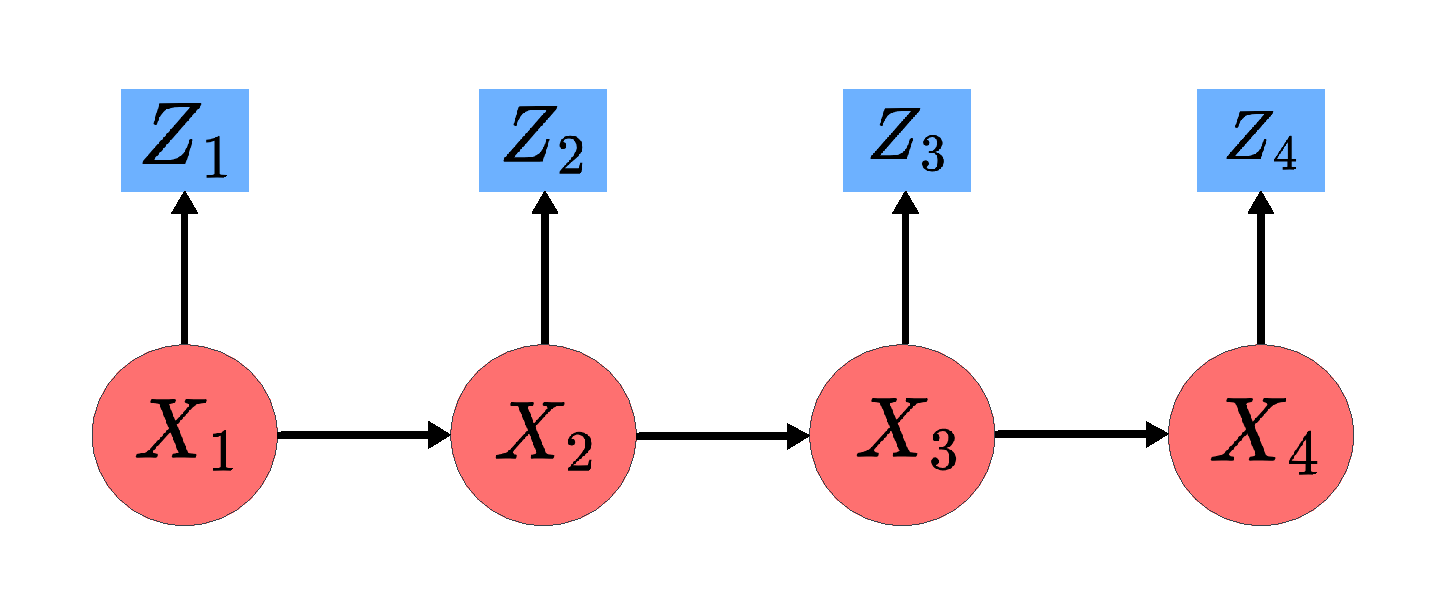
\includegraphics[width=0.5\linewidth]{img/BeyseNetAppendix}
	\caption{شبکه بیز معادل مربوط به مسئله مثال  تخمین حالت بیان‌شده}
	\label{fig:beysenetappendix}
\end{figure}

فرمول‌بندی احتمالاتی بیزی که تا کنون ذکر شده است، می‌تواند به صورت گرافیکی
با استفاده از شبکه‌های بیزی ارائه شود. یک شبکه بیزی
\footnote{\lr{BayesNet}}
یک مدل گرافیکی جهت‌دار است
که متغیرهای تصادفی به عنوان گره‌های آن و یال‌ها نمایانگر وابستگی‌ها (علت و معلول)
بین این گره‌ها هستند. به عبارت دیگر، یک شبکه بیزی می‌تواند توزیع احتمالی مشترک
را بر روی همه متغیرهای تصادفی به عنوان حاصل‌ضرب چگالی‌های شرطی تعریف کند. شکل~\ref{fig:beysenetappendix}
شبکه بیزی مربوط به سیستم غیرخطی مثال ما را نشان می‌دهد. توزیع احتمالی مشترک
مربوطه ممکن است به صورت زیر نوشته شود:
\begin{equation}
	p(X, Z) = p(x_1) p(x_2|x_1) p(x_3|x_2) p(x_4|x_3) \newline
	\times p(z_1|x_1) p(z_2|x_2) p(z_3|x_3) p(z_4|x_4)
\end{equation}
در این معادله، تکه اول اول نمایانگر مدل سیستم و تکه دوم
نمایانگر مدل‌های مشاهده است.

 توزیع مشترک در معادله
 \ref{eq:MAP}
 به توزیع پسین \(p(X|Z)\) با استفاده از فرمول احتمال شرطی زیر پیوند می‌خورد:
\begin{equation}
	p(X|Z) = \frac{p(X, Z)}{p(Z)}
\end{equation}
\(p(Z)\) در این معادله به عنوان یک عامل نرمال‌سازی عمل می‌کند، بنابراین \(p(X|Z)\) متناسب با توزیع مشترک \(p(Z, X)\) است. تخمین $MAP$ معادل خواهد بود با بیشینه‌سازی تابع درست‌نمایی \(l(X; Z)\) که متناسب با \(p(Z, X)\) است:
\begin{equation}
	l(X; Z) \propto p(Z|X)
\end{equation}
بدین‌ترتیب خواهیم داشت:
\begin{equation}
	X^{MAP} = \arg\max_X l(X; Z)
\end{equation}

علاوه بر این، می‌توانیم مقیاس‌های ثابت را در احتمالات شرطی معادلات A.3 و A.4 حذف کنیم و تابع درستنمایی \(l(X; Z)\) را به صورت زیر بنویسیم:

\begin{equation}
	l(X; Z) = l(x_1) l(x_2|x_1) l(x_3|x_2) p(x_4|x_3) \\
	\times l(z_1|x_1) l(z_2|x_2) l(z_3|x_3) l(z_4|x_4)
\end{equation}

که در آن:

\begin{equation}
	l(X; z) = \exp \left\{ -\frac{1}{2} \|g(X) - z \|_R^2 \right\}, \quad l(X_{k+1}; X_k) = \exp \left\{ -\frac{1}{2} \|f(X_k, u_k) - X_{k+1}\|_Q^2 \right\}
\end{equation}

بنابراین، تابع درستنمایی که باید بیشینه شود، حاصل‌ضرب تجزیه‌شده‌ای از توابع درستنمایی کوچکتر است. در حالی که توزیع احتمالی مشترک در معادله A.6 به بهترین شکل با استفاده از یک شبکه بیزی توصیف می‌شود، تابع درستنمایی تجزیه‌شده در معادله A.8 ممکن است به بهترین شکل با یک گراف فاکتور نمایش داده شود.

یک گراف فاکتور \(G\) تجزیه یک تابع \(f(X)\) را به عنوان حاصل‌ضربی از فاکتورها \(f_i\) تعریف می‌کند. این یک مدل گرافیکی دو بخشی و بدون جهت با دو نوع گره است: گره‌های فاکتور \(f - i \in F\) و گره‌های متغیر \(x_i \in X\). یک یال \(e_{ij} \in E\) در گراف حضور دارد اگر و فقط اگر \(f_i\) تابعی از \(x_j\) باشد [15]. شکل A.2 گراف فاکتور متناظر با تابع درستنمایی در معادله A.8 را نشان می‌دهد. در این شکل، فاکتورهای زرد رنگ به درستنمایی‌های اندازه‌گیری اشاره دارند در حالی که فاکتورهای سیاه رنگ به مدل سیستم اشاره می‌کنند.
در نهایت، با استفاده از الگوریتم ML، مسئله MAP به یک مسئله LS غیرخطی تبدیل می‌شود.






%\begin{figure}
%	\centering
%	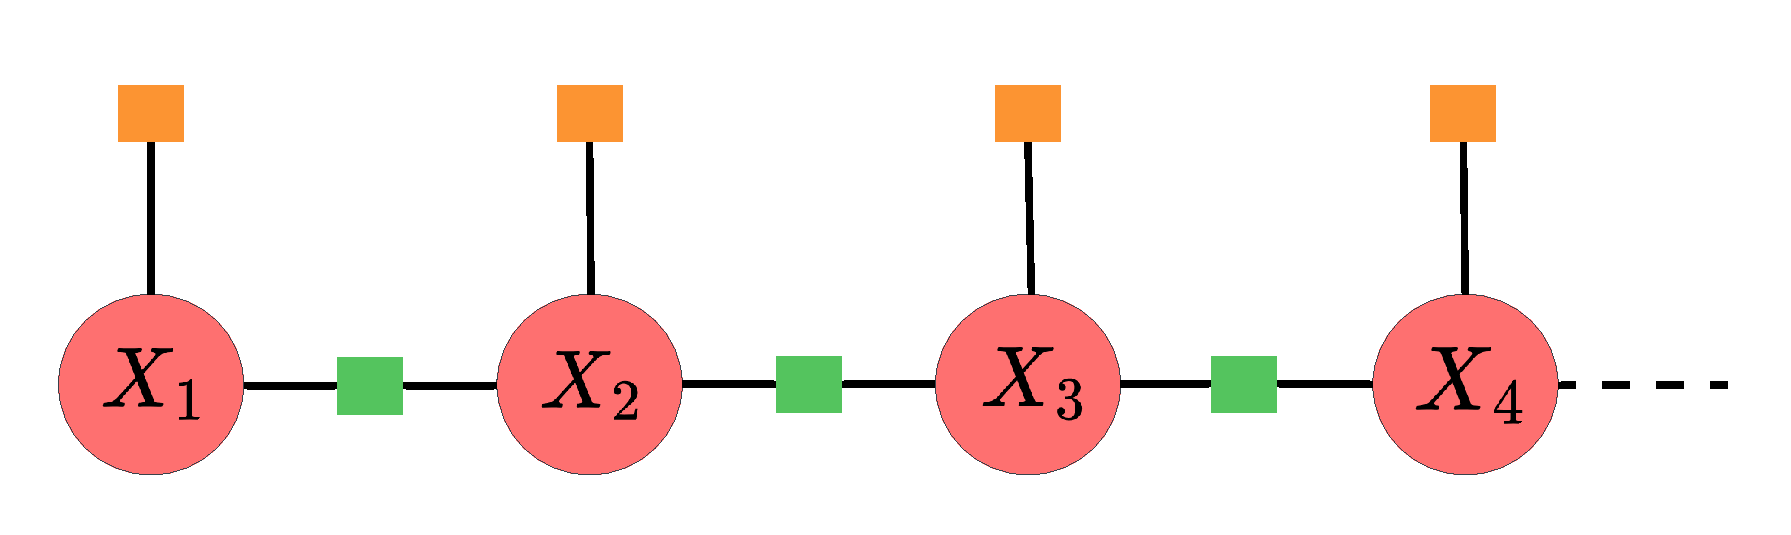
\includegraphics[width=0.4\linewidth]{img/StateEstimationFGAppendinx}
%	\caption{شبکه بیز معادل مربوط به مسئله مثال  تخمین حالت بیان‌شده}
%	\label{fig:stateestimationfgappendinx}
%\end{figure}
